\subsection{Teil 1-4}
%TODO Timo: Zusammenfassung von VL und Übung
\subsection{Teil 1}
\subsubsection{Grundlagen, Definition}
Informationssysteme sind unabhängig von Wirtschaft oder öffentlicher Verwaltung:
\textbf{zentrale, essenzielle Systeme zur Unterstützung von Menschen}
\par
Definition Infortmationssysteme:
\par
\textbf{Ein Informationssystem (Abkürzung IS; engl.: Information system) besteht aus Menschen und Maschinen (Rechner samt Software, Netzen, Kommunikationseinrichtungen), die Information erzeugen und/oder benutzen und die durch Kommunikationsbeziehungen miteinander verbunden sind.}
\par
Betriebliches Informationssystem unterstützt die Leistungsprozesse und Austauschbeziehungen innerhalb eines Betriebs sowie zwischen dem Betrieb und seiner Umwelt.
\par
\begin{itemize}
  \item rechnergestütztes Informationssystem zur Erfassung, Speicherung, Übertragung und/oder Transformation von Information
  \item operatives Informationssystems unterstützt Leistungsprozesse mit betrieblichen Anwendungsprogrammen. Aufgaben innerhalb von betrieblichen Funktionsbereichen (Beschaffung, Produktion, Vertrieb, Finanzwesen, Personalwirtschaft usw.) unterstützt, als auch Geschäftsprozesse, die diese Funktionsbereiche 
  \item Planungssystem unterstützt Führungskräfte eines Betriebs.
  \item Ein Kontrollsystem Überwachung der Einhaltung der Pläne durch Soll-Ist-Vergleiche und Hinweise auf notwendige Korrekturmaßnahmen
  \item Zusammengefasst werden Informationssysteme für Führungskräfte als Managementunterstützungssysteme bezeichnet.
\end{itemize}
\par
Integrierte Informationssysteme
\begin{itemize}
  \item horizontal integriertes Informationssystem verbindet Teilsysteme aus unterschiedlichen Funktionsbereichen auf einer Ebene.
  \item Ein vertikal integriertes Informationssystem verknüpft Teilsysteme des gleichen Funktionsbereichs auf verschiedenen Stufen, etwa ein System für die Abwicklung von Geschäftstransaktionen mit einem Büroinformationssystem und einem Managementunterstützungssystem 
\end{itemize}
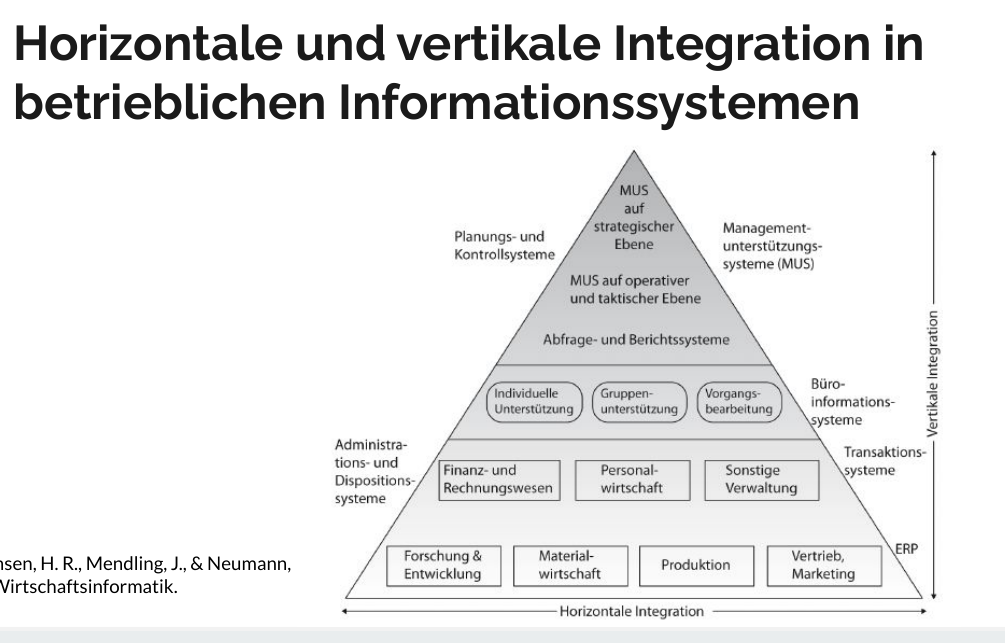
\includegraphics[width=0.8\textwidth]{assets/HoriVertIntegration.PNG}
\par
Ein modulares System ist ein System, dessen Subsysteme unter den Gesichtspunkten der Überprüfung der Funktionsfähigkeit, der Austauschbarkeit und der Arbeitsorganisation gebildet werden.

\subsubsection{Sozio-technische Systeme}
\par
Sozio-technische Systeme sind Systeme, bei denen eine technische und eine soziale Teil- komponente untrennbar voneinander zusammenspielen. Während das Verhalten der technischen Komponente eines Informationssystems durch Programmierung festgelegt wird, ist das Detailverhalten der sozialen Teilkomponenten weit weniger bestimmbar.
\par
\subsubsection{Schalenmodell nach Teubner}
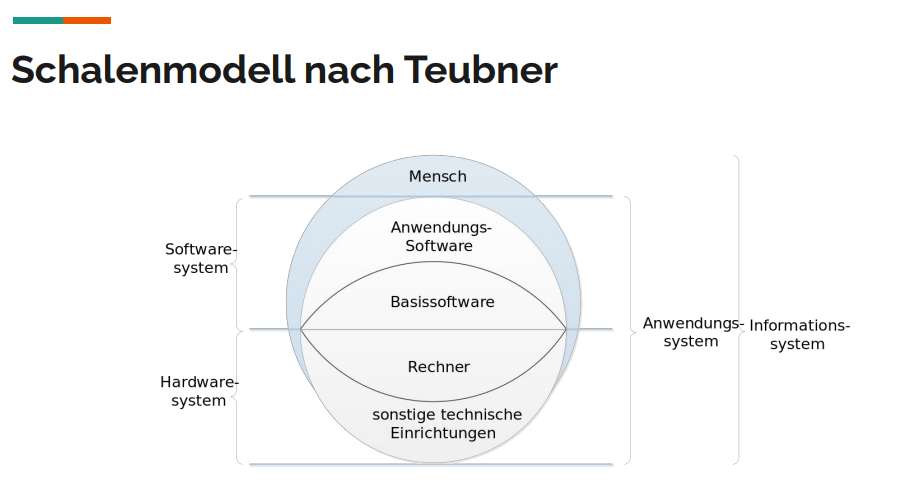
\includegraphics[width=0.8\textwidth]{assets/SchalenmodellTeubner.PNG}
\begin{itemize}
  \item Hauptaugenmerk auf den soziotechnischen Anteil des Systems.
  \item Technik aufgeteilt in Anwendungssoftware und Basissoftware, zusammengefasst als Softwaresystem
  \item Rechner und technische Einrichtungen, zusammengefasst als Hardwaresystem
  \item Der Mensch greift auf alle Ebenen des Systems zu.
  \item Das Grundziel des Systems, die Unterstützung betrieblicher Aufgaben liegt ideell im Hintergrund
  \item Aufgabe durch Anwendungssystem realisiert und liegt im Wert, der Lösung eines betrieblichen Problems, durch Zusammenspiel von Mensch und Technik mit vorgegebener Aufgabe entsteht.
\end{itemize}


\subsubsection{Offene Standards}
Unter einem offenen Standard versteht man einen Standard, der für alle Marktteilnehmer zugänglich ist (das heißt, veröffentlicht ist), kostenfrei genutzt und wiederverwendet werden kann. Meist werden offene Standards von gemeinnützigen Organisationen beschlossen, die allen interessierten Parteien Einflussnahme bei der Ausgestaltung und Weiterentwicklung der Standards ermöglichen
\subsubsection{Ziele betrieblicher Informationssysteme}
Drei Oberziele sind:
\begin{itemize}
  \item wirtschaftlich
  \item sozial
  \item ökologisch
\end{itemize}
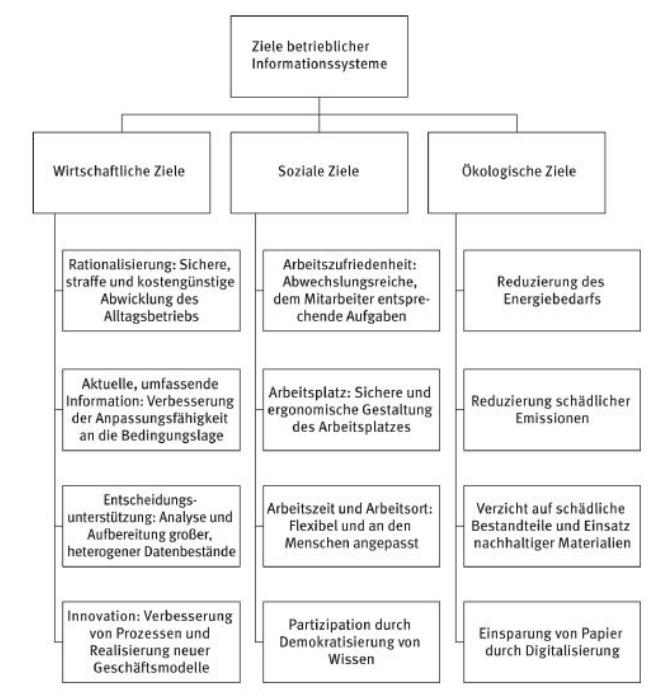
\includegraphics[width=0.8\textwidth]{assets/ZielebetrieblicherInfosysteme.PNG}
\subsubsection{Informationssysteme für die ÖV}
\begin{itemize}
  \item Begriff “Informationssysteme” wurde durch Wirtschaftsinformatik hauptsächlich für Betrieb geprägt, aber auch für Verwaltungen
  \item Berücksichtigung von Aspekte wie Barrierefreiheit, Inklusion, Zugänglichkeit (auch demografisch) bei Behörden von ausgeprägterer Wichtigkeit
  \item finanzielle und personelle Ressourcen unterschiedlich ÖV und Wirtschaft
  \item eher Gemeinwohlorientierung in ÖV als Gewinnorientierung in Wirtschaft
  \item Beispiele für Informationssysteme in ÖV sind: Fahrgastinformationssystem, Bürgerinformationssystem, Abfallkalender
\end{itemize}

\subsection{Teil 2}
\subsubsection{Trends: Vernetzung, Mobile, Cloud, Open Source}
\begin{itemize}
  \item Vernetzung: IT als digitale Spielwelt, soziale Netzwerke, Geschäftsmodelle sind E-Commerce, E-Business, E-Government\ldots.
  \item Mobile IT: Smartphonenutzung, Funktechnik, Displaytechnik; Beispiele sind E-mail, Banking, Informationssuche, Unterhaltung und Spiele
  \item Cloud: Servicemodelle (Softwareaas, PlatformaaS, InfrastructureaaS)(Anwendung / Hardware / Plattform), Cloud-Anbieter und Datenschutz bzw. Datensicherheit
  \item Open Source: öffentlicher Quelltext zur Veränderung, Einsicht und meist kostenloser Nutzung (z.B. Linux in Münchener Verwaltung)
\end{itemize}

\subsubsection{Hype-Cycle kennen und mit Trends umzugehen wissen}

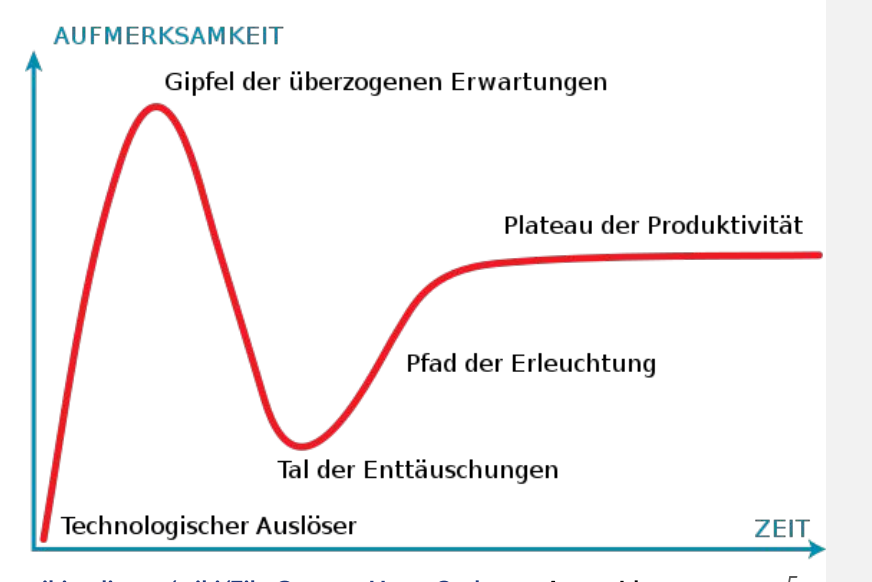
\includegraphics[width=0.8\textwidth]{assets/HypeCycle.PNG}
IT-Trends schlagen sich irgendwann auch - positiv oder negativ - in Anforderungen und Systemen (Hype-Cycle berücksichtigen).
\par
Aktualität und das “immer am Ball” bleiben wichtig, um technologisch auf der Höhe der Zeit zu bleiben, aber auch nicht alles mitzumachen
\par Status von Verwaltungen: oft keine early adopter, sondern späte Nutzung (ggf. zu spät)
\par Trendthemen (Arbeitsweisen, Technologien, Hardware, Nutzarten) kommen und gehen seit jeher - Fortschritt nötig und wichtig

\subsection{Teil 3}
\subsubsection{Grundlagen, Definition Geschäftsprozesse}
Geschäftsprozesse oft sehr individuell, Generalisierung über typische Geschäftsprozesse möglich (Bestellung, Ausschreibung, Beschwerde, Beantragung)
\par
Aufgaben in Teilaufgaben zerlegen
\par
Definition:
\begin{itemize}
  \item komplexer, aus mehreren Funktionen bestehender Arbeitsablauf zur Erledigung einer betrieblichen Aufgabe
  \item Funktionen stehen zueinander in zeitlich-sachlogischen Zusammenhang und tragen zu (betriebswirtschaftlichem) Ziel bei
  \item verschiedene Teilnehmer arbeitsteilig mit Durchführung einzelner Funktionen betraut; sie gebrauchen Informationen und Vorleistungen, um ein Produkt oder eine Dienstleistung zu erstellen
\end{itemize}
Prinzipien des Geschäftsprozessmanagements sind Koordination, Geschäftsprozesstyp und Geschäftsfall.
\par
Koordination: aufeinander Abstimmen von Aktivitäten, die von unterschiedlichen Aktoren (Personen oder automatisierte Teilprozesse) mit dem Ziel der Effizienz durchgeführt werden
\par
Geschäftsprozesstyp (business process type): beschreibt allgemeinen Arbeitsablauf für eine Klasse von gleichartigen Geschäftsfällen
\par
Geschäftsfall (case): ist eine Geschäftsprozessinstanz (business process instance); ein Geschäftsfall entspricht konkretem, spezifischem Arbeitsablauf gemäß den Vorgaben des Geschäftsprozesstyps
\par
\subsubsection{Effektivität und Effizienz}
Effektivität (Wirksamkeit) und Effizienz (Wirtschaftlichkeit) als wichtige Maße für die Qualität
\par
Qualität von Geschäftsprozessen hat wichtigen Einfluss auf Qualität der betrieblichen Leistungen
\subsubsection{BPMN als Modellierungssprache (lesen und beschreiben können)}
Business Process Model and Notation
\par
Abbildung von Prozessen unter Berücksichtigung von Akteuren, Aktionen und Abhängigkeiten
\subsubsection{Lebenszyklus des Geschäftsprozessmanagements}
Geschäftsprozessmanagement (business process management): Gesamtheit aller Aufgaben und Maßnahmen, die darauf abzielen, Geschäftsprozesse effizienter und effektiver zu machen
Lebenszyklus
\begin{itemize}
  \item Aufgaben des Geschäftsprozessmanagements als ein sich wiederholender Ablauf
  \item umfasst Identifikation, Erhebung, Analyse, Verbesserung, Einführung und Überwachung von Prozessen
\end{itemize}
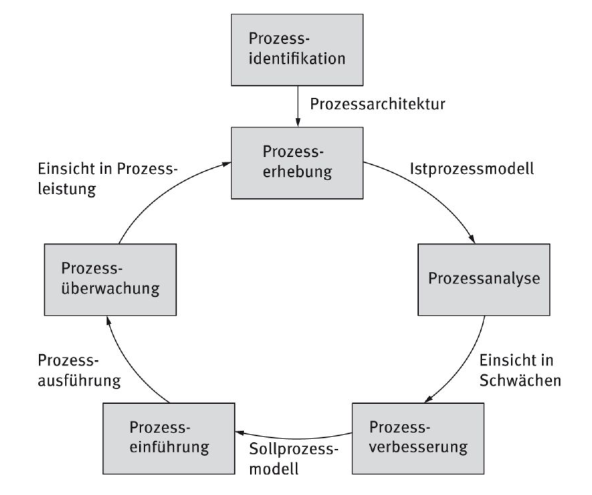
\includegraphics[width=0.8\textwidth]{assets/LebenszyklusGPM.PNG}
\subsubsection{Gestaltung von Geschäftsprozessen (Erheben, Analysieren, Verbessern)}
Prozesse Erheben:
\begin{itemize}
  \item Sammlung von Informationen zu einem Prozess und dessen Aufbereitung in Form eines Istmodells
  \item Istprozessmodell beschreibt Geschäftsprozess so, wie er aktuell tatsächlich von den Prozessteilnehmern (!) ausgeführt wird
  \item Prozesse sind arbeitsteilig organisiert
  \item Verwendung geeigneter Terminologie
  \item Methoden: bestehende Dokumentation/Beobachtung/Interviews/Workshops
\end{itemize}
Prozesse Analysieren:
\begin{itemize}
  \item systematisches Aufspüren von Schwachstellen eines Prozesses und deren Ursachen
  \item Wertbeitragsanalyse (value-added analysis) ordnet jede Funktion eines Prozesses den Kategorien wertschöpfend, geschäftsdienlich und nicht wertschöpfend zu
  \item Ursache-Wirkungs-Diagramm (cause-effect diagram) dient der Analyse von Ursachen für ein Problem und unterscheidet dabei die Ursachenkategorien Mensch, Maschine, Milieu, Material, Methode und Messung
\end{itemize}
Ursache-Wirkungs-Diagramm:
\par
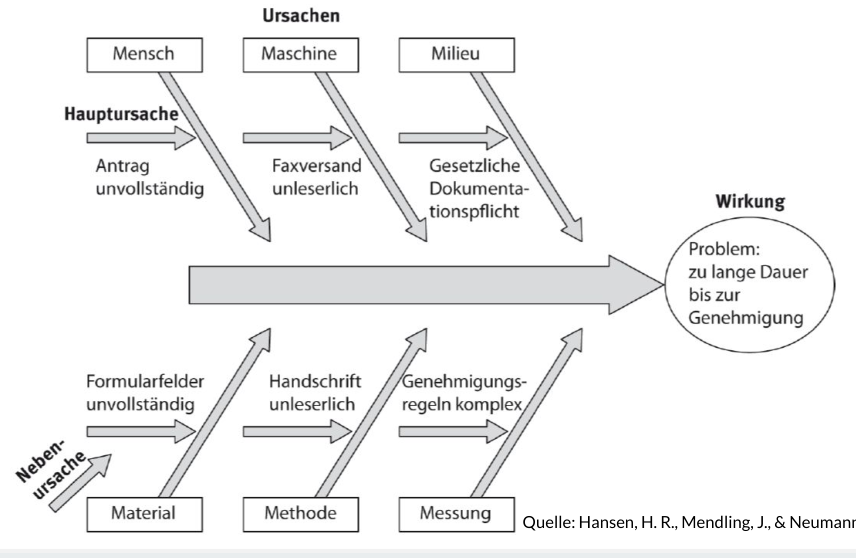
\includegraphics[width=0.8\textwidth]{assets/UrsacheWirkungDIa.PNG}
\par
Prozesse Verbessern:
\begin{itemize}
  \item betrachtet bestehenden Geschäftsprozess und dessen Schwachstellen und entwickelt systematisch Vorschläge für die Verbesserung
  \item Dimensionen Durchlaufzeit, Kosten, Qualität und Flexibilität sind oft derart miteinander verknüpft, dass Verbesserungen in der einen Dimensionen eine Verschlechterung in einer anderen nach sich ziehen
  \item Redesign-Heuristik beschreibt konkrete Maßnahme zur Umgestaltung eines Geschäftsprozesses, die mit Erwartung einer Verbesserung in zumindest einer Dimension verbunden ist
  \item Sollprozessmodell (Resultat der Redesign-Heuristik) beschreibt Geschäftsprozess so, wie er in Zukunft gestaltet sein sollte
  \item Sollprozessmodell ist eine Vorlage für die Umsetzung von Prozessverbesserungen 
\end{itemize}
Beispiele: 
\par
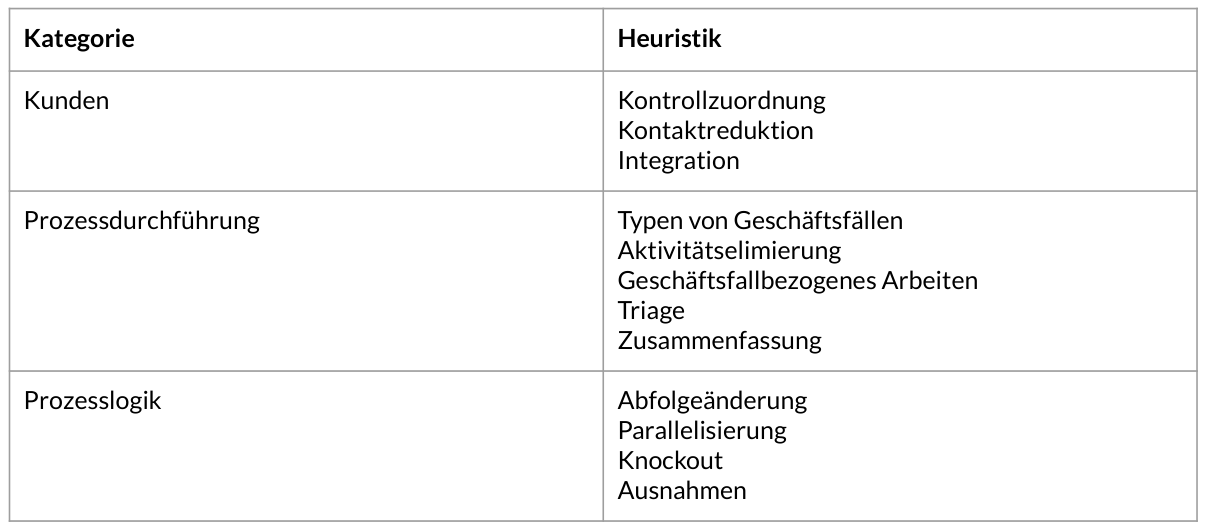
\includegraphics[width=0.8\textwidth]{assets/BeispieleHeuristiken.PNG}

\subsection{Teil 4}
\subsubsection{Grundlagen}

Unter Modellierung (engl.: modeling) versteht man die vereinfachende und zweckorientierte Abbildung eines Sachverhalts. Der Begriff Abbildung lässt sich hier sowohl als Verrichtung als auch als Ergebnis verstehen. Als Verrichtung beschreibt Modellierung den Vorgang, einen Sachverhalt nach Maßgabe eines bestimmten Zwecks zu verkürzen und abzubilden. Als Ergebnis erhält man aus diesem Vorgang ein Modell (engl.: model)
\par
Charaktaristika:
\begin{itemize}
 \item Abbildungscharakter (Referenz auf Bezugspunkt)
 \item Vereinfachungseigenschaft (Modell einfacher als Original) 
 \item Zweickorientierung (durch Zweckdefinition kann Modellierer entscheiden was relevant)
\end{itemize}

Prinzipien (Ziel: vereinfachende Darstellung eines komplexen Systems):
\begin{itemize}
 \item Partitionierung (Zerlegung eines großen Sachverhalts in kleinere isolierbare Teilbereiche)
 \item Projektion (Betrachtung eines Sachbereichs aus bestimmter Perspektive / Sichtweise von Personengruppen und Rollen einnehmen)
 \item Abstraktion (Ausblenden von Details zur Konzentration auf wesentliche Sachverhalte)
\end{itemize}

Arten von Modellen an Beispiel U-Bahn:
\begin{itemize}
 \item Istmodell Sachverhalt aktueller Zustand (U-Bahn-Plan für Fahrgäste)
 \item Sollmodell, entwerfender Charakter, Zustand in Zukunft sein soll (Darstellung eines möglichen Streckennetzes)
 \item Referenzmodell abstrahieren von konkretem Sachverhalt, versucht Lösung für allgemeine Problemstellung darzustellen  (im Allgemeinen die Kreuzung zweier U-Bahn-Linien in Form der Gleisstränge)
\end{itemize}

Anwendungsfälle:
\begin{itemize}
 \item Organisationsbezogene Anwendungsfälle (Betrieb mit Hilfe von Modellen darstellen/Dokumentationszwecke, Organisationsverbeserung)
 \item Entwicklung und Anpassung von Informationssystemen (klassische Entwicklung / Aspekte und Perspektvien erfassen, Auswahl von Standardsoftware)
 \item Referenzmodell abstrahieren von konkretem Sachverhalt, versucht Lösung für allgemeine Problemstellung darzustellen  (im Allgemeinen die Kreuzung zweier U-Bahn-Linien in Form der Gleisstränge)
\end{itemize}
\subsubsection{BPMN}
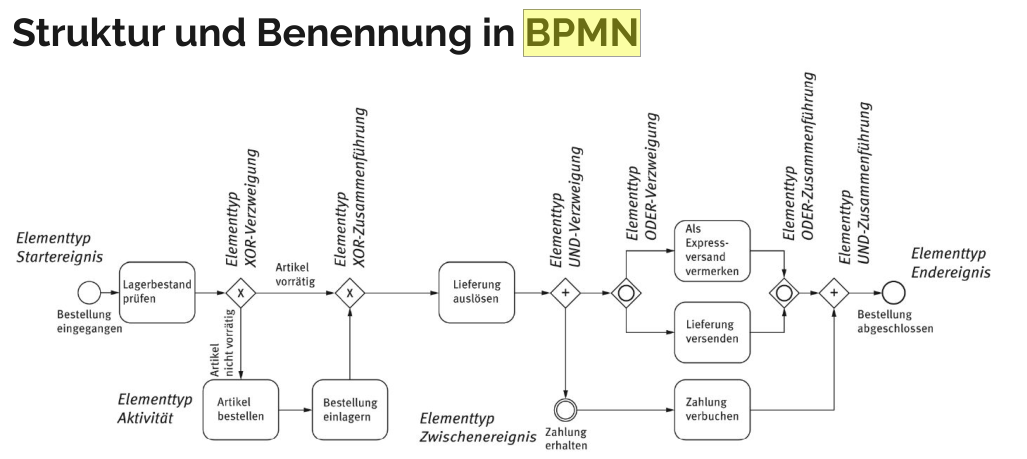
\includegraphics[width=0.8\textwidth]{assets/BPMN.PNG}
\subsubsection{ER-Modell sollte bekannt sein}
Das Entity-Relationship-Modell (kurz: ER-Modell, engl.: entity relationship model) definiert die Datenelemente (engl.: entity) mit ihren Attributen, die in einem Informationssystem gespeichert werden sollen


